We present various mathematical expressions, which can be computed more efficiently
than initial formulation would suggest. This section is finalized with  
approximations of partition function. 

\subsection{Snippets}

There are given matrices $A \in \mathbb{R}^{n \times m}$, $B \in \mathbb{R}^{m \times k}$. 
Goal is to compute 
\begin{align*}
	\sum AB = \sum_{i = 1}^n \sum_{k = 1}^m \sum_{j = 1}^k A_{i, k} B_{k, j} 
\end{align*}
Naive algorithm would take $O(nmk)$ time. However, we have found with our framework 
computation giving the same expression in time O(n(k + m)) :

\begin{verbatim}
	sum(sum(A .* repmat(sum(B, 2), [1, n])'))
\end{verbatim}

Empirical tests indicate that aforementioned computation is indeed faster (Figure \ref{ab}).

\begin{figure}[h]
\centering
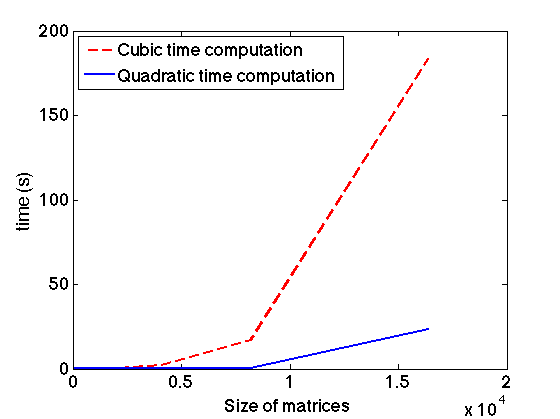
\includegraphics[scale=0.3]{img/ab.png}
\caption{Computation time for $\sum AB$ using standard algorithm vs using inferred optimal algorithm.}
\label{ab}
\end{figure}


Similarly, we found quadratic time computation instead of cubic for similar expressions like : 
\begin{align*}
	\sum ABC\\
	\sum ABCD\\
	\sum AA^T\\
	\sum AA^TA\\
\end{align*}

One could automatically analyze large code repositories to find other expressions, which are computed inefficiently. 
Our optimization rules could be placed into compilers.

\subsection{Partition function approximation}

As we shown in Section \ref{partitionfunction}, we can manually find $O(n^2)$ computation of $g(x \rightarrow x^k, W)$ for $k = 1, 2$ 
instead of native exponential time computation. By use of
our framework, we found rules for $k = 3, 4, 5$ (however for $k = 4, 5$ we found only computation in $O(n^3)$ time). 
Finding computation for higher degree polynomials is expensive.
Table \ref{grammars} shows time necessary to
generate all the rules. It is worth to note, that grammar can be evaluated just once, and the resulting coefficients can 
be stored. Process of partition function approximation involves step of computation discovery only once. However, due to limited computation power
we analyzed only powers $k \leq 5$. As we noted in Section \ref{agenda}
it is extremely important and interesting to find pattern how to generate $g(x \rightarrow x^k, W)$ for $k \geq 6$.


Table \ref{eval} shows number of terms necessary to derive $g(x \rightarrow x^k, W)$ for various $k$. Plot \ref{approximations} shows 
how well partition function is approximated with finite Taylor expansion. Finally, plot \ref{time_approx} 
compares computation time of derived rules to the computation time of naive exponential time algorithm.

\begin{table}
\tiny
\centering
\begin{tabular}{|l||l|l|}
\hline\hline
Order & Size of grammar & Computation time (s) \\
\hline\hline
2 & 5 & 17 \\
3 & 15 & 188 \\
4 & 48 & 2535\\
5 & 139 & 31320 \\
\hline
\end{tabular}
\caption{Table summarizes size and computational time for grammars of specific degree.}
\label{grammars}
\end{table}

\begin{table}
\tiny
\centering
\begin{tabular}{|l|l|l|}
\hline\hline
Order & Number of terms & Complexity \\
\hline\hline
2 & 4 & $O(n^2)$\\
3 & 5 & $O(n^2)$\\
4 & 21 & $\mathbf{O(n^3)}$\\
5 & 30 & $\mathbf{O(n^3)}$\\
\hline
\end{tabular}
\caption{Table summarizes complexity of computation of $g(x \rightarrow x^k, W)$.} 
\label{eval}
\end{table}

\begin{figure}[h]
\centering
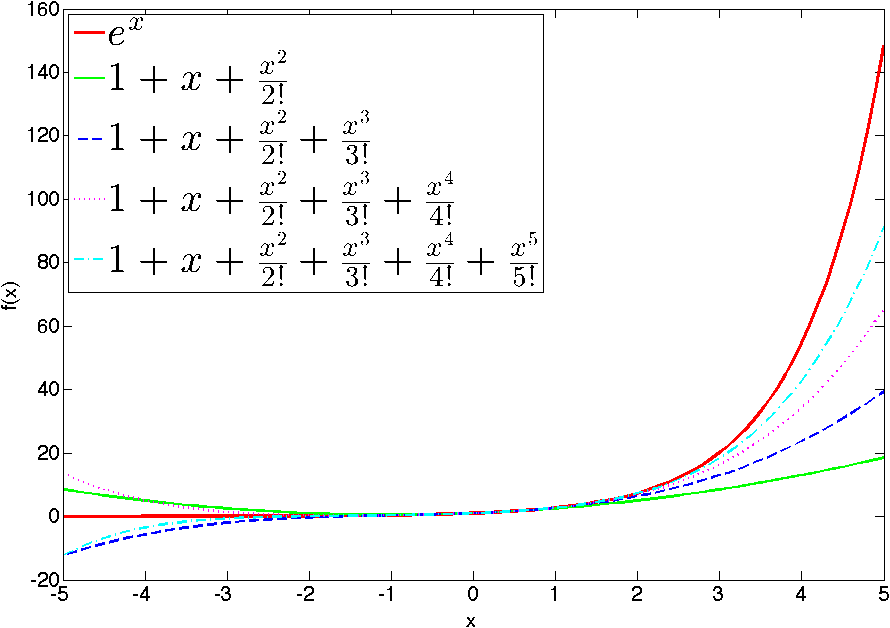
\includegraphics[scale=0.2]{img/approximations.png}
\caption{Comparison of approximations with various number of Taylor terms.}
\label{approximations}
\end{figure}



\begin{figure}[h]
\centering
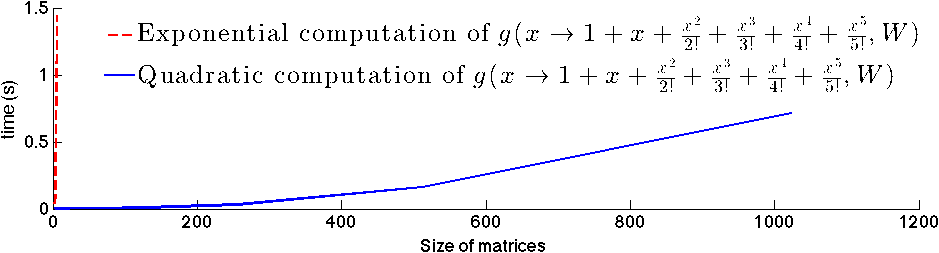
\includegraphics[scale=0.24]{img/time_approx.png}
\caption{Comparison of computation time for naive exponential time algorithm vs our optimized derivation.}
\label{time_approx}
\end{figure}


